\documentclass[11pt,a4paper,fontset=fandol]{ctexart}

\usepackage[a4paper,top=2.25cm,bottom=2.2cm,left=2.15cm,right=2.15cm]{geometry}
\usepackage{amsmath,amssymb}
\usepackage{booktabs}
\usepackage{caption}
\usepackage{enumitem}
\usepackage{fancyhdr}
\usepackage{float}
\usepackage{graphicx}
\usepackage{microtype}
\usepackage{tabularx}
\usepackage{xcolor}
\usepackage[hidelinks]{hyperref}
\usepackage{titlesec}

\graphicspath{{figures/readme/}}
\setlength{\parindent}{2em}
\setlength{\parskip}{0.35em}
\setlist[itemize]{leftmargin=1.8em,itemsep=0.25em,topsep=0.35em}
\setlist[enumerate]{leftmargin=1.8em,itemsep=0.25em,topsep=0.35em}

\definecolor{navy}{HTML}{17365D}
\definecolor{blue}{HTML}{4C78A8}
\definecolor{orange}{HTML}{F58518}
\definecolor{green}{HTML}{54A24B}
\definecolor{lightblue}{HTML}{EAF1F8}
\definecolor{lightgray}{HTML}{F4F5F6}
\definecolor{darkgray}{HTML}{455A64}

\titleformat{\section}{\Large\bfseries\color{navy}}{\thesection}{0.7em}{}
\titleformat{\subsection}{\large\bfseries\color{darkgray}}{\thesubsection}{0.7em}{}
\titlespacing*{\section}{0pt}{1.4em}{0.6em}
\titlespacing*{\subsection}{0pt}{1.1em}{0.4em}

\pagestyle{fancy}
\fancyhf{}
\fancyhead[L]{\small\color{darkgray}Execution Algorithm Research}
\fancyhead[R]{\small\color{darkgray}TWAP / Forecast VWAP / POV}
\fancyfoot[C]{\small\color{darkgray}\thepage}
\renewcommand{\headrulewidth}{0.3pt}
\renewcommand{\footrulewidth}{0pt}
\setlength{\headheight}{14pt}

\captionsetup{font=small,labelfont={bf,color=navy},textfont={color=darkgray}}
\renewcommand{\arraystretch}{1.25}

\newcommand{\algoTWAP}{\textcolor{blue}{\textbf{TWAP}}}
\newcommand{\algoVWAP}{\textcolor{orange}{\textbf{Forecast VWAP}}}
\newcommand{\algoPOV}{\textcolor{green}{\textbf{POV}}}
\newcommand{\keybox}[1]{%
  \begin{center}
    \fcolorbox{navy}{lightblue}{\parbox{0.91\textwidth}{\vspace{0.35em}#1\vspace{0.35em}}}
  \end{center}}

\begin{document}

\begin{titlepage}
  \thispagestyle{empty}
  \vspace*{1.4cm}
  \noindent{\color{navy}\rule{\textwidth}{1.2pt}}\par\vspace{1.1cm}
  {\fontsize{25}{32}\selectfont\bfseries\color{navy}
    TWAP、Forecast VWAP 与 POV\\[0.25cm]
    执行算法比较研究\par}
  \vspace{0.8cm}
  {\Large\color{darkgray}执行节奏、成本分布与 Regime 敏感性}
  \vspace{1.4cm}

  \begin{center}
  \begin{tabular}{rl}
    \textbf{研究标的：} & AAPL 5-minute OHLCV \\
    \textbf{样本期间：} & 2026-07-24 至 2026-07-31 \\
    \textbf{测试设计：} & Full-day fixed-Q + 60-minute Dynamic-Q \\
    \textbf{版本日期：} & 2026-08-26 \\
  \end{tabular}
  \end{center}

  \vfill
  \begin{center}
    \fcolorbox{navy}{lightgray}{%
      \parbox{0.84\textwidth}{
        \textbf{核心问题}\quad
        在相同母订单和执行约束下，时间驱动的 TWAP、预测成交量驱动的 Forecast VWAP、以及实时成交量驱动的 POV，分别表现出怎样的执行路径、完成时点、成本分布和市场状态敏感性？
      }}
  \end{center}
  \vfill
  \noindent{\small\color{darkgray}
    本报告用于执行算法研究与方法展示。结果来自本仓库的可复现 AAPL fixture 和简化成交模型，不构成投资建议或生产级 TCA 结论。}\par
  \vspace{0.8cm}
  \noindent{\color{navy}\rule{\textwidth}{1.2pt}}
\end{titlepage}

\section*{执行摘要}
\addcontentsline{toc}{section}{执行摘要}

本报告的结论不是某一种算法全面胜出，而是三种方法承担不同类型的执行风险。\algoTWAP{} 的路径最平滑、交易前可预测性最高，但忽略日内流动性曲线；\algoVWAP{} 利用交易前估计的 volume profile 调整节奏，其主要风险来自成交量曲线预测误差；\algoPOV{} 使用一根 bar 滞后的已观察成交量作反馈，完成时点最灵活，但成本分布更宽、完成风险更明显。

\keybox{\textbf{主要发现：}固定前 5 日训练、最后 1 日测试的 23 个重叠 Dynamic-Q 窗口中，Forecast VWAP 相对 TWAP 的 mean $\Delta IS$ 为 $+1.14$ bps、胜率为 26.1\%；滞后 POV 为 $-2.52$ bps、胜率为 52.2\%。3\% Q 下三种算法均完成；Q 提高至 15\% 时 POV 平均 completion 降至 60.9\%。}

单日固定母订单案例中，当日价格自 arrival 后明显下跌，arrival IS 主要反映成交时点与单日价格路径的交互，不应解释为算法 alpha。算法评价必须先明确 benchmark：贴近 market VWAP、降低 arrival shortfall、控制 modeled impact 和确保按时完成，是不同的目标。

\subsection*{结论总览}

\begin{table}[H]
\centering
\small
\begin{tabularx}{\textwidth}{p{2.4cm}XXX}
\toprule
\textbf{维度} & \textbf{TWAP} & \textbf{Forecast VWAP} & \textbf{POV} \\
\midrule
主要驱动 & 时间 & 预测成交量曲线 & 已观察市场成交量 \\
执行路径 & 最平滑、最确定 & 预先向预测高量时段倾斜 & 随实际放量快速调整 \\
主要风险 & 流动性错配 & Profile forecast error & 路径与完成时点风险 \\
当前样本 & 稳定 baseline & 与 TWAP 非常接近 & 尾部更宽、regime 敏感 \\
\bottomrule
\end{tabularx}
\end{table}

\clearpage
\tableofcontents
\clearpage

\section{数据与研究边界}

\subsection{数据口径}

研究使用 AAPL 5-minute OHLCV，共覆盖 2026-07-24 至 2026-07-31 的 6 个完整正常交易日。每个交易日保留 09:30 至 16:00 ET，共 78 根 bar；完整样本为 468 根 bar。

\begin{table}[H]
\centering
\small
\begin{tabularx}{0.96\textwidth}{p{3.3cm}X}
\toprule
\textbf{项目} & \textbf{设置} \\
\midrule
标的与频率 & AAPL，5-minute OHLCV \\
Full-day 测试 & 2026-07-31；前 5 日估计 Forecast VWAP profile \\
Dynamic-Q 测试 & 2026-07-31；固定使用此前 5 日估计 profile \\
数据文件 & \texttt{Data\_example/example.pkl}，可由公开 CSV 离线重建 \\
Volume 定义 & Provider-defined tick volume，不是 consolidated share volume \\
\bottomrule
\end{tabularx}
\end{table}

选择 5 分钟频率，是为了在日内成交量形状和 bar-level 噪声之间取得折中。数据时间对齐采用 bar 所属交易日和日内 slot：历史日相同 slot 用于估计 profile，测试日 volume 不进入 Forecast VWAP 的预测曲线。

\subsection{研究边界}

当前 fixture 的 volume 口径足以验证算法结构、整数守恒和统一成交模型，但不能将 POV participation 解释为严格的股票市场成交份额。报告中的 3\% Dynamic-Q 也只是相对 tick volume 的研究标准化。生产研究需要授权的 consolidated trades/quotes、明确的 auction 和 odd-lot 口径，以及可审计的数据修订规则。

\section{算法定义与经济含义}

设母订单总量为 $Q$，执行窗口有 $N$ 个 bar，$V_i$ 为第 $i$ 个 bar 的市场成交量，$R_i$ 为进入该 bar 时的剩余母订单量，$L$ 为 lot size。

\subsection{TWAP：时间驱动的确定性基准}

\begin{equation}
q_i^{\mathrm{TWAP}} \approx \frac{Q}{N}.
\end{equation}

TWAP 给每个时间桶相同权重，并通过 largest-remainder 方法处理整数余量，使计划量严格等于 $Q$。它交易前完全确定、容易监控，也是比较其他 schedule 的自然 baseline。其代价是忽略 U-shaped liquidity：当市场低量时，固定子单会对应更高的实际参与率。

\subsection{Forecast VWAP：预测日内成交量曲线}

先将每个训练日的成交量归一化为日内占比：

\begin{equation}
s_{d,i}=\frac{V_{d,i}}{\sum_jV_{d,j}},\qquad
\hat p_i=\frac{\operatorname{median}_d(s_{d,i})}
{\sum_k\operatorname{median}_d(s_{d,k})},\qquad
q_i^{\mathrm{VWAP}}\approx Q\hat p_i.
\end{equation}

本项目实现的是 \textbf{Forecast-Profile VWAP}，不是提前知道测试日成交量的 realized-volume oracle。按日归一化避免绝对高量日主导 profile，中位数降低异常日影响。其优势是把计划量向预期高流动性时段移动；风险是历史曲线可能无法代表测试日。

\subsection{POV：实际成交量驱动的反馈策略}

\begin{equation}
q_i^{\mathrm{POV}}
=\min\!\left(R_i,\left\lfloor\frac{\rho V_{i-1}}{L}\right\rfloor L\right),
\qquad q_1^{\mathrm{POV}}=0,
\qquad \rho=10\%.
\end{equation}

POV 用前一根已完成 bar 的成交量更新子单：观察到放量后加速，观察到缩量后减速。默认一根 bar 滞后消除了用同 bar 完整 volume 决策的 look-ahead。若窗口市场量不足，它可以留下未完成量。

\begin{table}[H]
\centering
\small
\begin{tabularx}{\textwidth}{p{2.2cm}p{2.6cm}p{2.8cm}XX}
\toprule
\textbf{算法} & \textbf{主要驱动} & \textbf{完整计划能否预知} & \textbf{主要优势} & \textbf{主要风险} \\
\midrule
TWAP & 时间 & 能 & 简单、稳定、透明 & 忽略流动性形状 \\
Forecast VWAP & 预测 profile & 能 & 匹配预期市场节奏 & Profile forecast error \\
POV & Lagged observed volume & 不能 & 适应已观察放量和缩量 & 反馈延迟与完成风险 \\
\bottomrule
\end{tabularx}
\end{table}

\clearpage
\section{实验设计与评价指标}

\subsection{Full-day fixed-Q：用于解释执行形态}

Full-day 案例固定为 AAPL、2026-07-31、BUY 5,000 shares、09:30 至 16:00 ET。三种算法面对同一母订单和统一成交约束，用于展示 per-bar schedule、累计完成路径、价格路径及单日 TCA 结果。这一层实验具有直观解释力，但只有一个交易日，不能用于稳定排名算法。

\subsection{Dynamic-Q：用于控制订单难度}

Dynamic-Q 固定使用前 5 个 session 训练，并在最后 1 日生成 23 个相互重叠的 60-minute 窗口；每个窗口包含 12 根 5-minute bar，每 15 分钟滚动一次。另生成 6 个不重叠窗口作为稳健性对照。每个窗口的母订单设置为：

\begin{equation}
Q_w=\left\lfloor 3\%\times\sum_i V_{w,i}\right\rfloor.
\end{equation}

样本中 $Q_w$ 范围为 170 至 734，中位数为 315。该设计让不同窗口的订单量与窗口成交量同比例变化，从而近似控制相对订单难度。不过，它使用完整窗口的 realized volume，是 ex-post research normalization，不是实盘可提前获得的 sizing 规则。

\subsection{Implementation shortfall 与方向}

对于 BUY 订单，arrival implementation shortfall 定义为：

\begin{equation}
IS=10^4\frac{P_{\mathrm{fill}}-P_{\mathrm{arrival}}}
{P_{\mathrm{arrival}}}.
\end{equation}

数值越低越好。报告图表使用包含显式费用的 net IS，CSV 同时给出不含费用的 gross price shortfall；两种口径不混用。算法相对 TWAP 的差值为 $\Delta IS=IS_{\mathrm{algo}}-IS_{\mathrm{TWAP}}$，因此 $\Delta IS<0$ 表示被比较算法优于 TWAP。所有算法都接受统一的 20\% bar-volume hard cap；计划量未成交时会 carry forward。

\begin{table}[H]
\centering
\small
\caption{Dynamic-Q 总体结果}
\begin{tabular}{lrrrr}
\toprule
\textbf{Algorithm} & \textbf{Mean IS} & \textbf{Mean $\Delta IS$} & \textbf{Win rate} & \textbf{Completion} \\
\midrule
TWAP & -29.46 bps & 0.00 bps & -- & 100.0\% \\
Forecast VWAP & -28.32 bps & +1.14 bps & 26.1\% & 100.0\% \\
POV & -31.98 bps & -2.52 bps & 52.2\% & 100.0\% \\
\bottomrule
\end{tabular}
\end{table}

\clearpage
\section{实证结果：Full-day fixed-Q}

\begin{figure}[H]
\centering
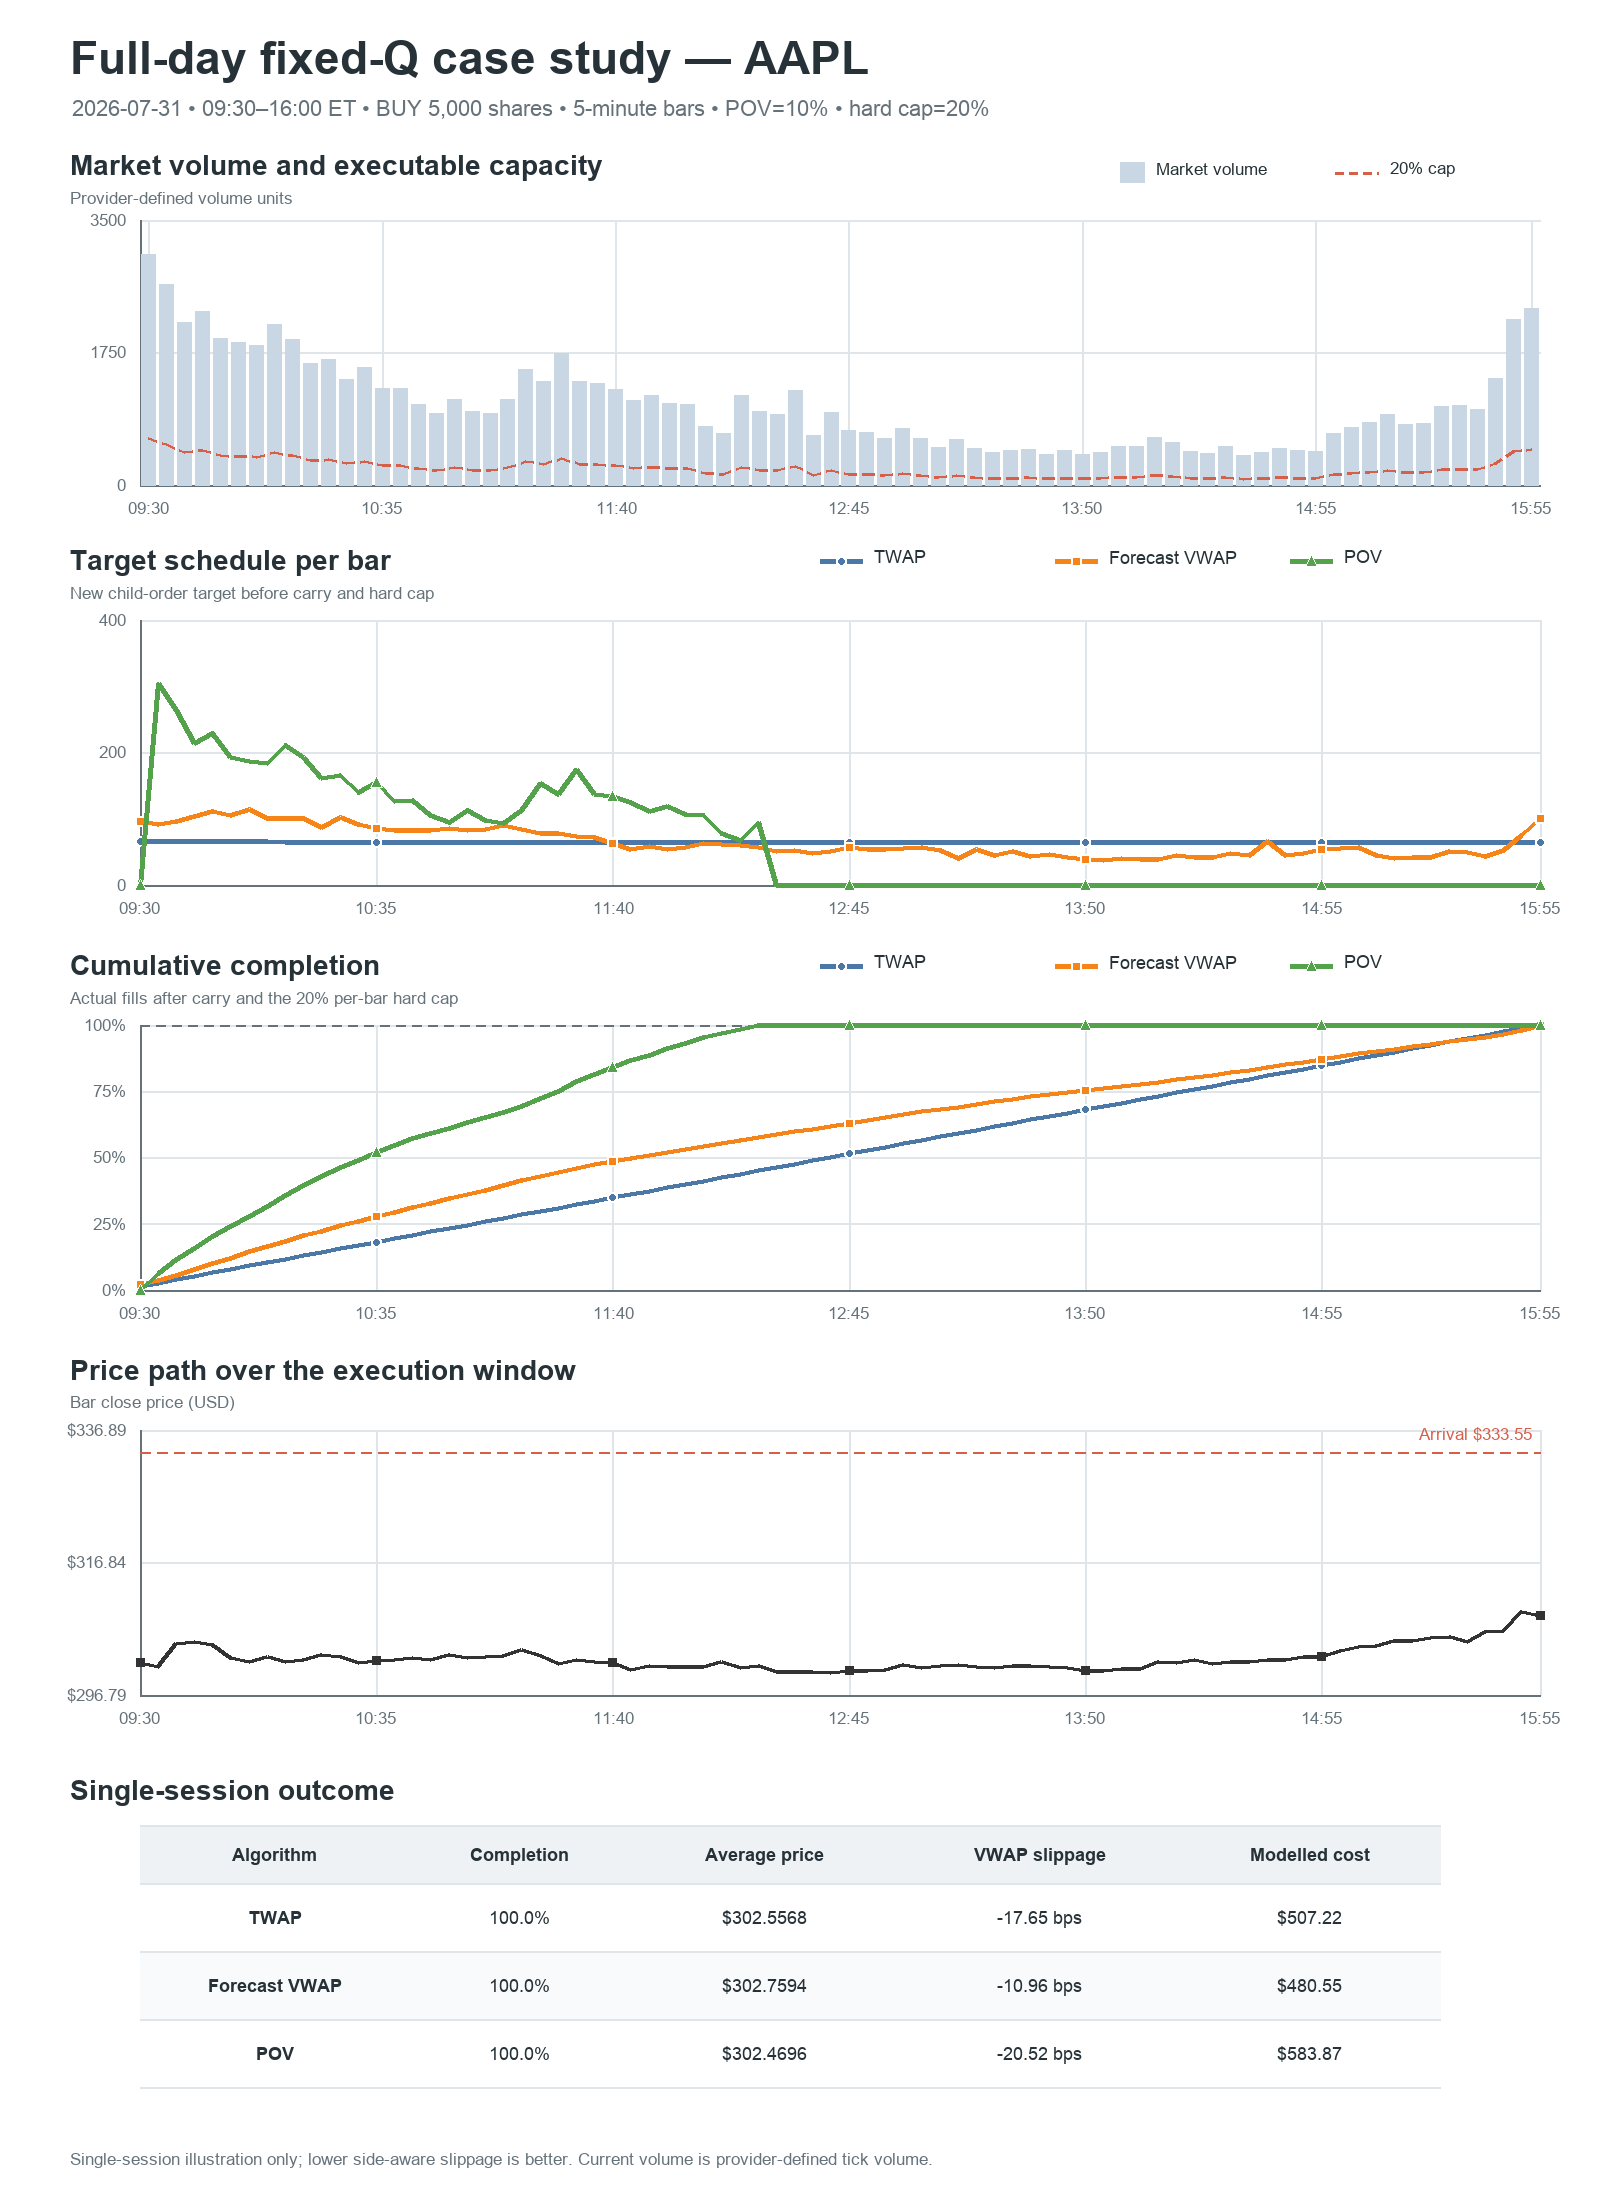
\includegraphics[width=0.90\textwidth,height=0.79\textheight,keepaspectratio]{00_full_day_case_study.png}
\caption{AAPL 全日固定母订单执行对比。上至下依次为市场成交量、per-bar schedule、累计完成路径、价格路径与结果表。}
\label{fig:fullday}
\end{figure}

\clearpage
\subsection{路径差异}

图 \ref{fig:fullday} 给出三种算法最直观的区别。\algoTWAP{} 每 bar 目标接近常数，累计成交量接近直线；\algoVWAP{} 根据历史 profile 在预测高量时段多做、低量时段少做；\algoPOV{} 首 bar 不使用未来信息，在观察到开盘放量后快速成交并明显提前完成。

\begin{table}[H]
\centering
\small
\caption{Full-day fixed-Q 结果}
\begin{tabular}{lrrrr}
\toprule
\textbf{Algorithm} & \textbf{Completion} & \textbf{Avg fill} & \textbf{VWAP slippage} & \textbf{Modelled cost} \\
\midrule
TWAP & 100.0\% & 302.5568 & -17.66 bps & \$507.22 \\
Forecast VWAP & 100.0\% & 302.7594 & -10.97 bps & \$480.55 \\
POV & 100.0\% & 302.4696 & -20.52 bps & \$583.87 \\
\bottomrule
\end{tabular}
\end{table}

当天价格从 arrival 后明显下跌，arrival IS 主要被市场路径主导。因果化后的 POV 在本日具有最低成交均价和最低 VWAP slippage，Forecast VWAP 的模型化 spread、impact 与 fee 合计最低。成交价格、VWAP tracking 和模型成本不会自动给出同一排名。

\keybox{\textbf{解释原则：}单日结果用于展示执行形态，而不是证明某算法持续优于另一算法。价格路径主导的 timing benefit 必须与算法自身的 spread、impact 和 completion risk 分开理解。}

\subsection{60-minute 单窗口示例}

\begin{figure}[H]
\centering
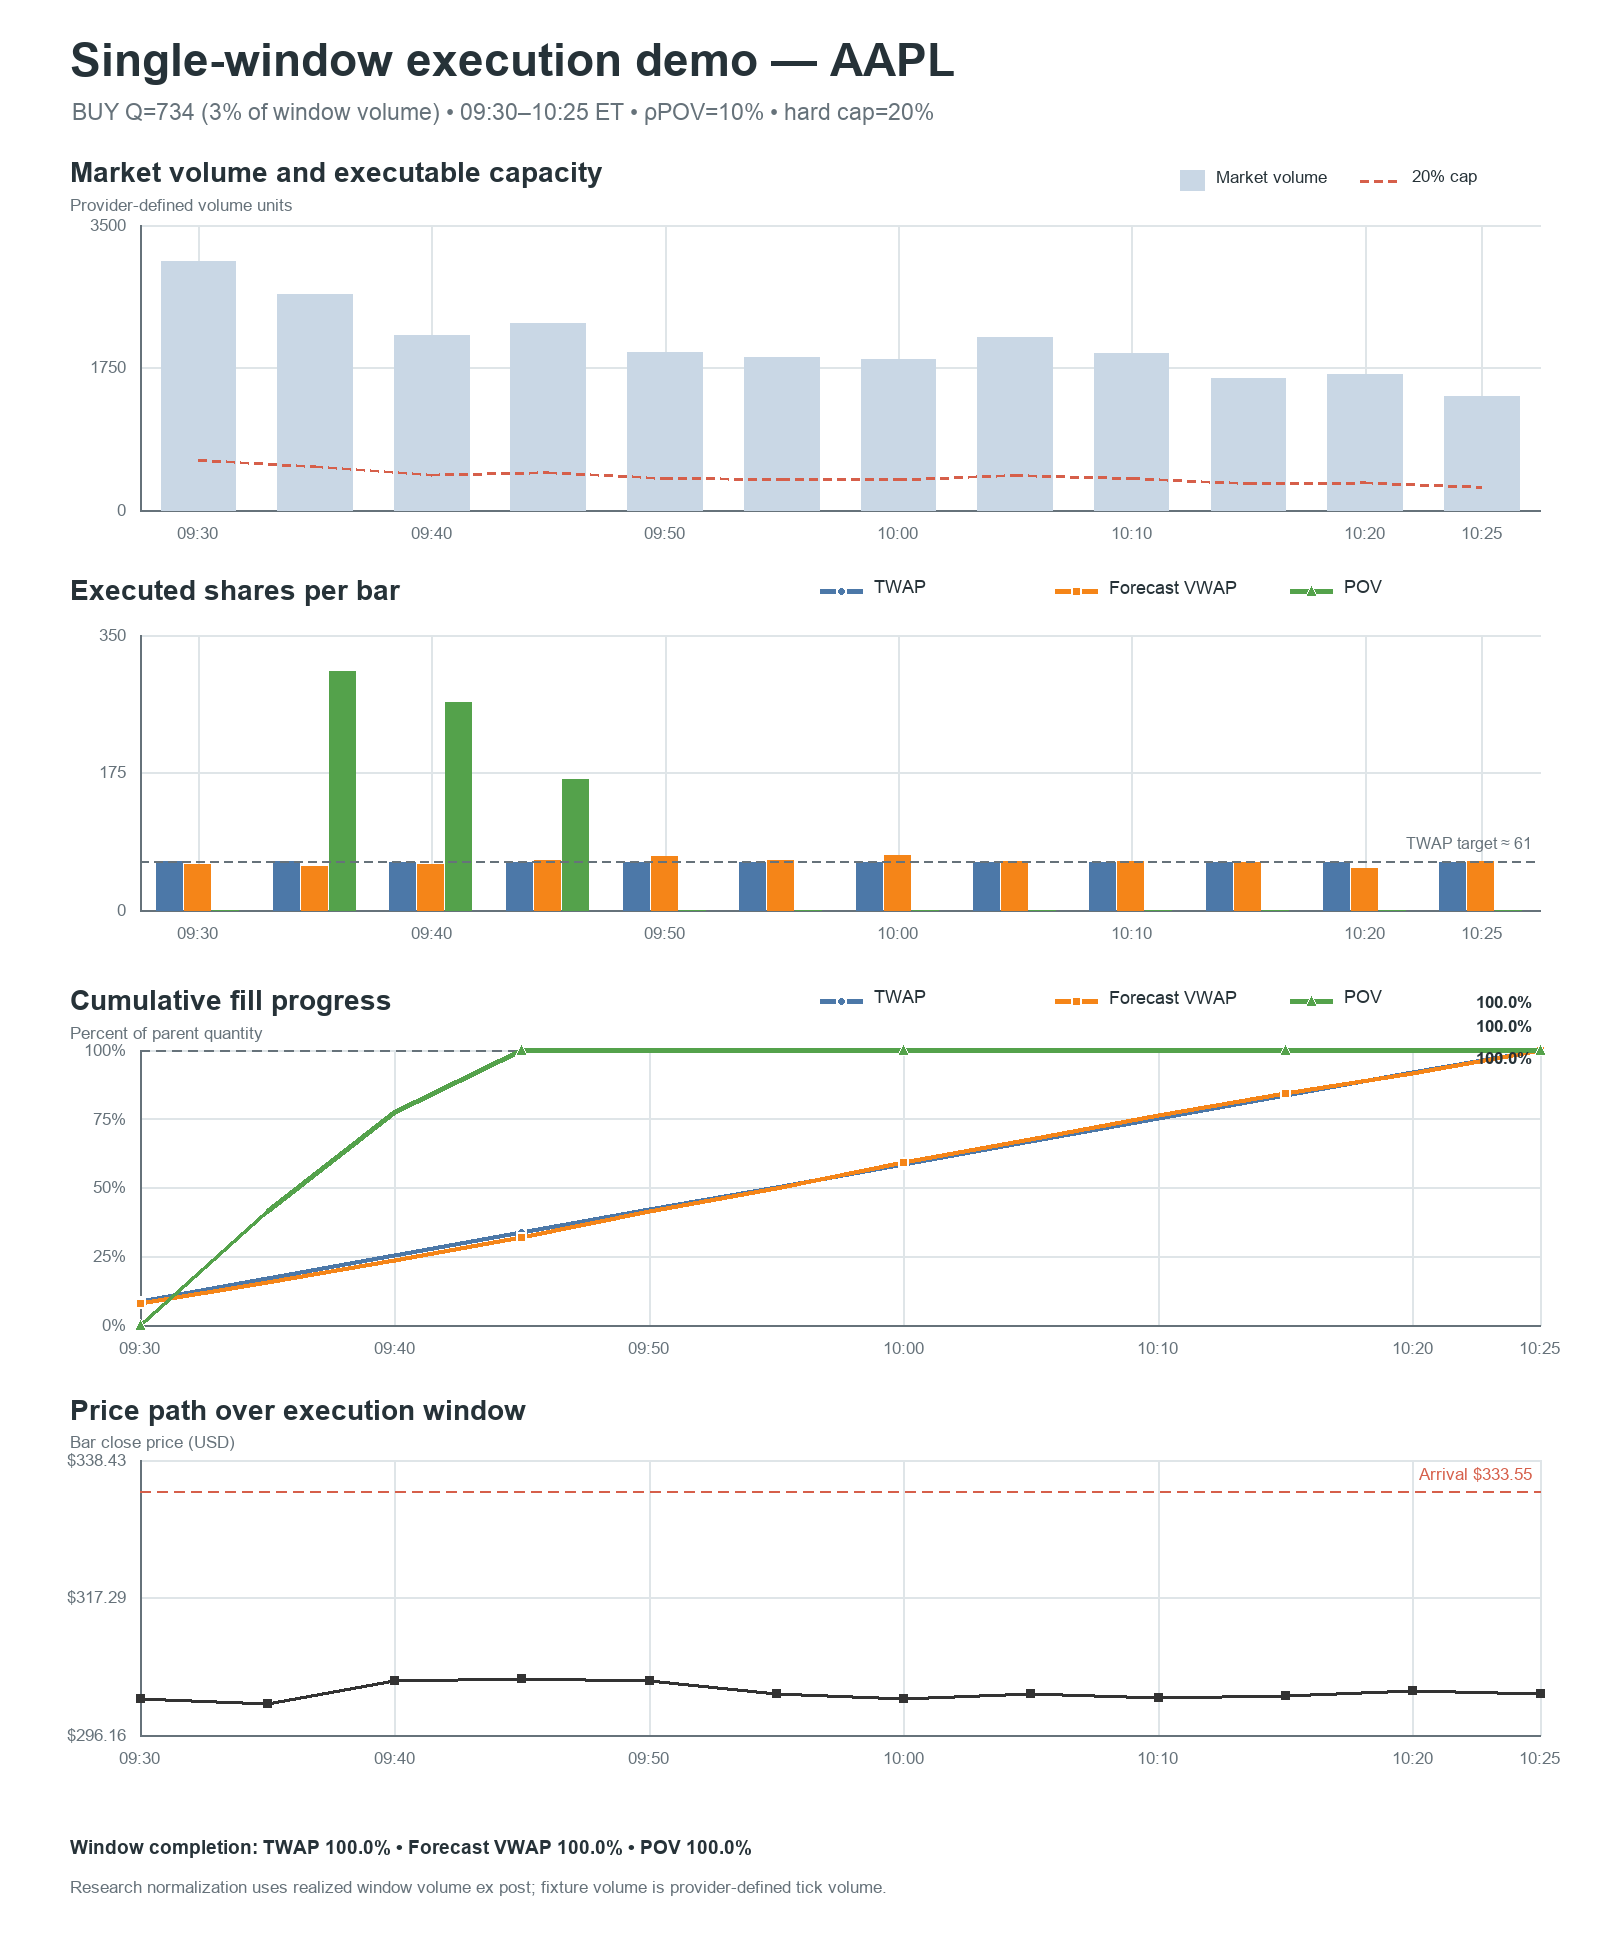
\includegraphics[width=0.79\textwidth,height=0.58\textheight,keepaspectratio]{01_single_window_demo.png}
\caption{Dynamic-Q 单窗口执行示例，$Q=734$。}
\label{fig:single}
\end{figure}

在图 \ref{fig:single} 中，三种算法均完成订单，但 TWAP 将交易均匀延伸到窗口末，Forecast VWAP 只做温和的 profile 倾斜，POV 首 bar 不交易，随后对已观察到的开盘放量作反馈并快速完成。

\clearpage
\section{实证结果：Dynamic-Q 分布比较}

\subsection{相对 TWAP 的 \texorpdfstring{$\Delta IS$}{Delta IS} 分布}

\begin{figure}[H]
\centering
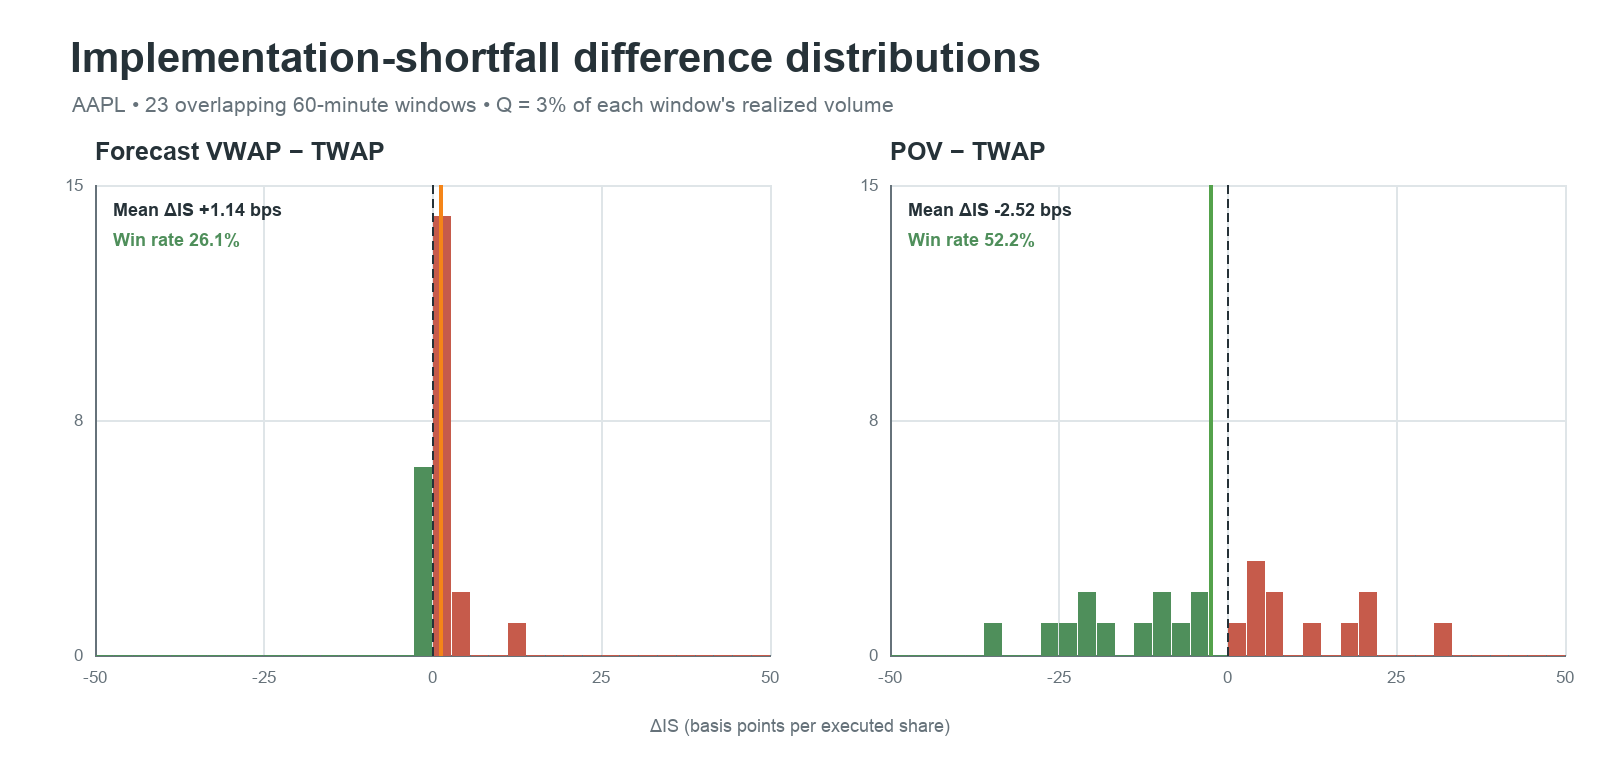
\includegraphics[width=0.94\textwidth]{02_delta_is_distribution.png}
\caption{Forecast VWAP 与 POV 相对 TWAP 的 implementation-shortfall 差值分布。小于 0 表示优于 TWAP。}
\label{fig:delta}
\end{figure}

图 \ref{fig:delta} 显示 Forecast VWAP 的差值紧密集中在 0 附近，意味着这些短窗口中它与 TWAP 的执行时点通常接近。Forecast VWAP 的 mean $\Delta IS$ 为 $+1.14$ bps、median 为 $+0.54$ bps、胜率为 26.1\%。

POV 的分布更宽、尾部更明显。其 median $\Delta IS$ 为 $-3.41$ bps，mean 为 $-2.52$ bps，胜率为 52.2\%。这种差异来自滞后 POV 对窗口内成交量顺序和价格路径的反馈：同样的窗口总量，如果放量发生在不同价格阶段，成交时点就会明显变化。

\subsection{为什么分布集中仍然有研究意义}

Forecast VWAP 与 TWAP 的 $\Delta IS$ 密集在 0 附近并不是绘图错误，而是实验结构的结果：窗口只有 60 分钟、订单只占窗口 volume 的 3\%、三种算法都在 20\% hard cap 下完整成交；同时，短窗口内历史 profile 的倾斜程度有限。23 个窗口都来自同一测试日且 75\% overlap，不可视为独立统计样本。

\clearpage
\section{Regime 分析}

\begin{figure}[H]
\centering
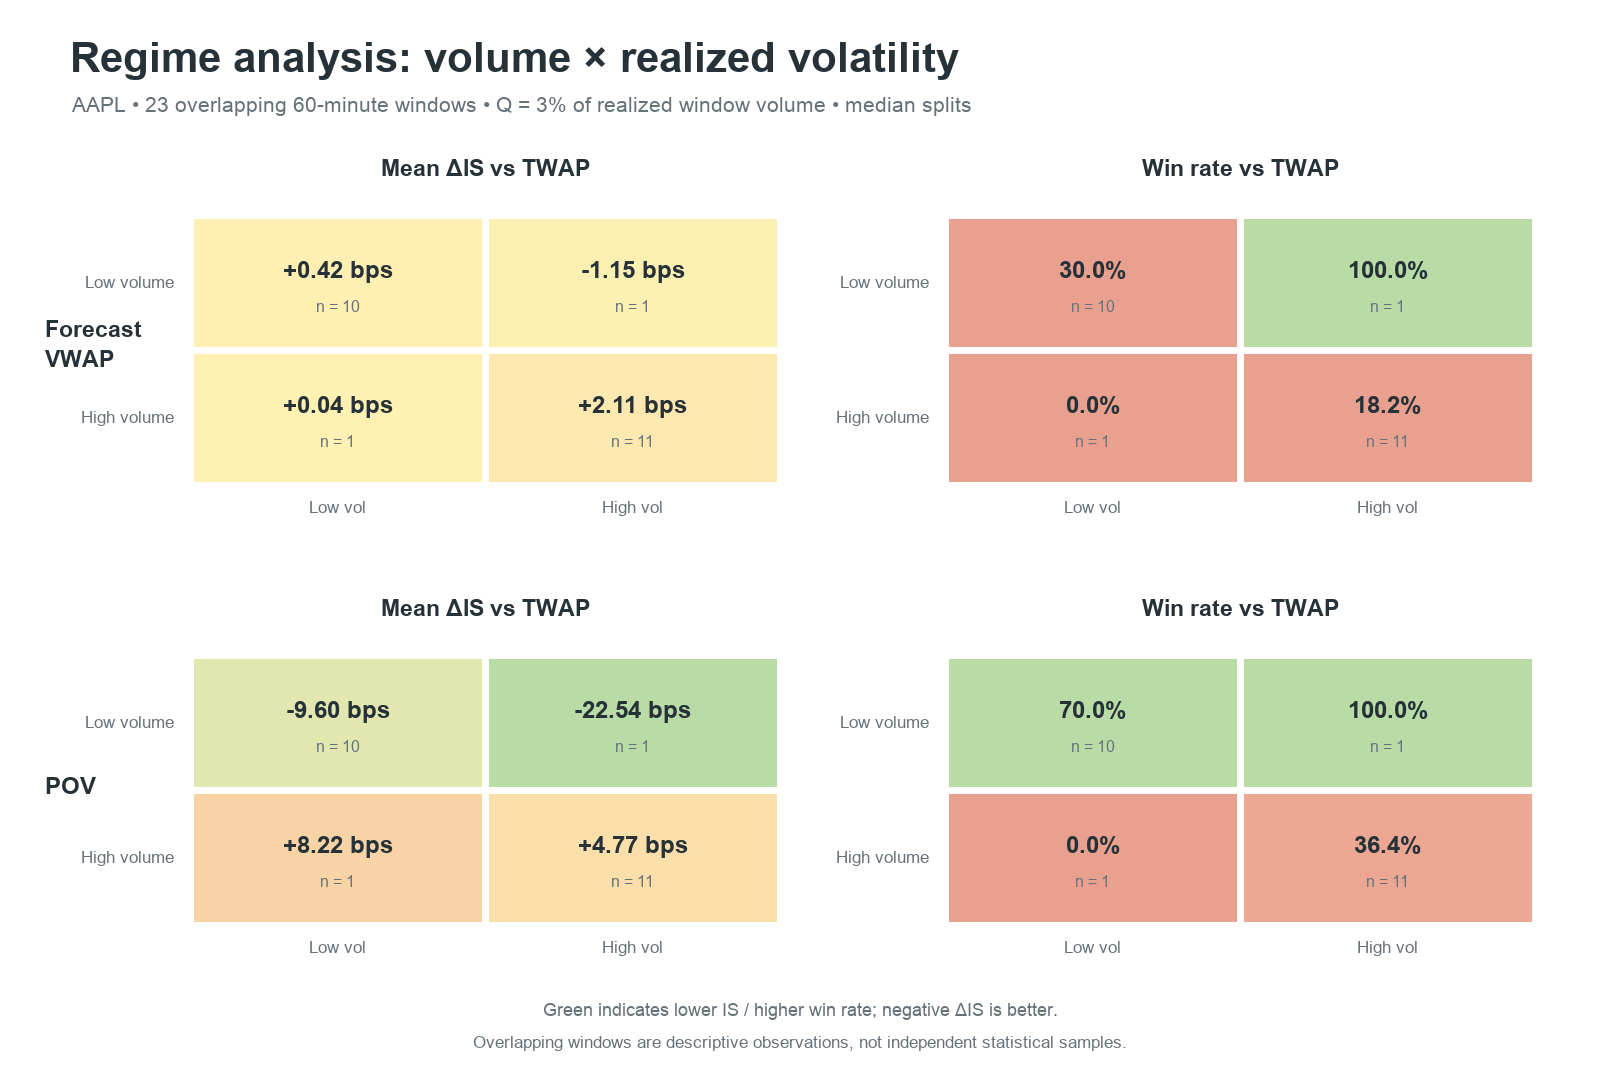
\includegraphics[width=0.96\textwidth]{03_regime_heatmap.png}
\caption{按 window volume 与 realized volatility 中位数划分的四种 regime。}
\label{fig:regime}
\end{figure}

\subsection{Forecast VWAP：平均差异较小，预测误差仍有条件性}

Forecast VWAP 在 low-volume/low-vol 与 high-volume/high-vol regime 的 mean $\Delta IS$ 分别为 $+0.42$ 和 $+2.11$ bps。两个非对角格各只有 1 个窗口，因此不能从这些格子的胜率作 regime 推断。

\subsection{POV：Regime 敏感性明显更强}

POV 在 low-volume/low-vol regime 的 mean $\Delta IS$ 为 $-9.60$ bps；在 high-volume/low-vol 和 high-volume/high-vol 中分别为 $+8.22$ 和 $+4.77$ bps。一个可能机制是滞后反馈把成交集中到放量之后的价格阶段，但这只是解释性推断，并非因果识别。

图中所有 regime 的 completion 都是 100\%。热力图只能提示条件性，不能构成可外推的 regime 证据。

\clearpage
\section{总体 IS 分布与完成率}

\begin{figure}[H]
\centering
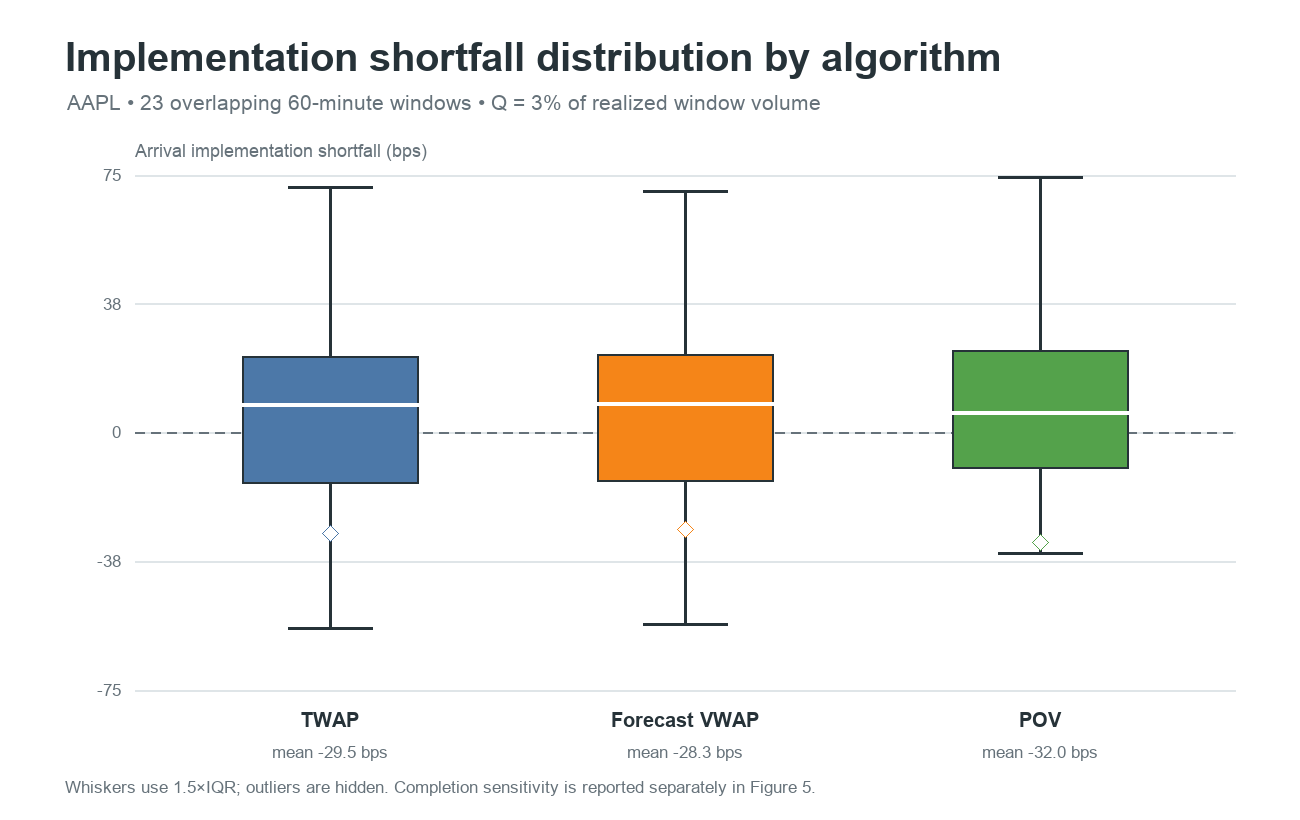
\includegraphics[width=0.72\textwidth]{04_is_distribution_by_algorithm.png}
\caption{三种算法在 23 个 Dynamic-Q 窗口中的 implementation-shortfall 分布。Whisker 使用 $1.5\times IQR$，隐藏 outlier。}
\label{fig:box}
\end{figure}

TWAP 与 Forecast VWAP 的箱体高度重叠。POV 的中心和离散程度有所不同，来自其滞后反馈的完成路径。三组 mean IS 分别为 $-29.46$、$-28.32$ 和 $-31.98$ bps，并被同一测试日开盘窗口的市场移动明显影响，不能被解释为算法 alpha。

\begin{figure}[H]
\centering
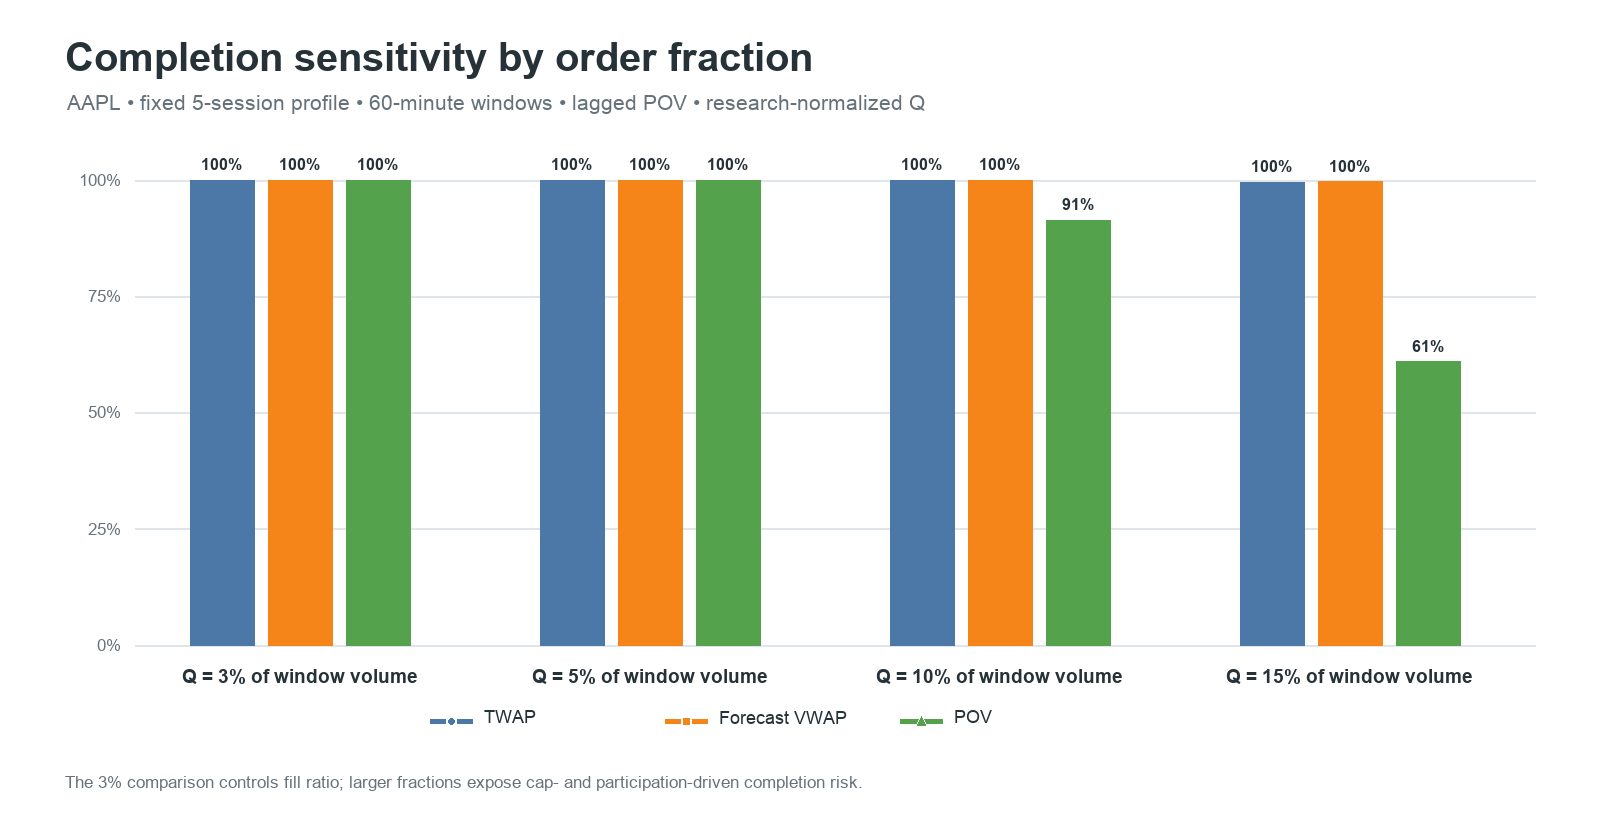
\includegraphics[width=0.80\textwidth]{05_completion_rate.png}
\caption{Q 占窗口 volume 3\%--15\% 时的平均 completion sensitivity。}
\label{fig:completion}
\end{figure}

3\% 和 5\% Q 下三种算法均完成；10\% Q 时 POV 平均 completion 降至 91.3\%，15\% 时降至 60.9\%，而 TWAP 与 Forecast VWAP 在 15\% 时约为 99.5\% 与 99.6\%。这说明 carry 只滚动已经产生但受 cap 限制的 target，并不会替 POV 强制调度全部母订单。

\clearpage
\section{综合判断与算法选择}

\begin{table}[H]
\centering
\small
\caption{三种算法的研究总结}
\begin{tabularx}{\textwidth}{p{2.7cm}XXX}
\toprule
\textbf{维度} & \textbf{TWAP} & \textbf{Forecast VWAP} & \textbf{POV} \\
\midrule
执行节奏 & 最平滑、最可预测 & 向预测高量时段倾斜 & 对已观察放量作滞后反馈 \\
完成时点 & 通常接近窗口末 & 通常接近窗口末 & 可提前，也可能因低量延迟 \\
当前样本 & 稳定 baseline & 与 TWAP 接近，局部小幅改善 & 分布更宽，regime 敏感更强 \\
主要风险 & 流动性错配 & Volume-profile forecast error & 反馈延迟、路径与完成风险 \\
适用目标 & 按时间均匀执行 & 跟随预期市场节奏 & 近似维持市场参与率 \\
\bottomrule
\end{tabularx}
\end{table}

\subsection{汇报时应如何表述}

\begin{enumerate}
  \item \textbf{先说明 benchmark。} 单日的 VWAP tracking、arrival IS 和 modeled cost 给出不同排名；arrival IS 会强烈依赖价格路径。
  \item \textbf{同时汇报 full-day 与 Dynamic-Q。} 前者回答“一笔固定订单如何执行”，后者回答“控制订单难度后的成本分布如何”，二者不能互相替代。
  \item \textbf{同时汇报 mean、median、win rate 和 completion。} 同时提供 3\% 主比较和更大 Q 的 completion sensitivity。
  \item \textbf{避免给出全局排名。} 当前结果支持“风险来源不同”和“表现具有 regime 条件性”，不支持“某算法永久最好”。
\end{enumerate}

\keybox{\textbf{最终结论：}TWAP 承担流动性错配风险，Forecast VWAP 承担预测风险，POV 承担路径和完成时点风险。实际选择应由客户 benchmark、订单占 ADV、完成约束、volume forecast 可信度与 urgency 共同决定。}

\section{研究限制与下一步}

\begin{enumerate}
  \item \textbf{样本不足。} 当前只有 AAPL 和 6 个交易日；主比较的 23 个窗口来自同一天且存在 75\% overlap，另有 6 个非重叠窗口，均不足以做显著性推断。
  \item \textbf{Volume 口径有限。} Tick volume 不是 consolidated shares，POV rate、Dynamic-Q 与 impact 只适合方法展示。
  \item \textbf{Forecast VWAP 较简单。} Profile 固定使用前 5 日中位数，没有 weekday、event、regime conditioning 或实时 reforecast。
  \item \textbf{成交模型简化。} 有 bar VWAP 时优先使用，否则回退 HLC/3；默认 spread、平方根临时 impact 和 fee 仍未模拟永久冲击、order book、queue、venue 与 adverse selection。
  \item \textbf{Dynamic-Q 是 ex-post 归一化。} 生产部署应改用客户预先给定的母订单、ADV 或 forecast window volume。
\end{enumerate}

下一步应换用授权的 consolidated trades/quotes，扩展到多标的和更长 walk-forward 历史，分离 market movement 与 execution cost，并对 volume forecast、POV completion risk 和 impact 参数进行稳定性检验。

\section*{文件与复现}
\addcontentsline{toc}{section}{文件与复现}

\begin{itemize}
  \item 算法与成交模型：\texttt{algo\_exec.py}
  \item 图表生成器：\texttt{figures/generate\_readme\_figures.py}
  \item Full-day 汇总：\texttt{figures/readme/full\_day\_summary.csv}
  \item Dynamic-Q 汇总：\texttt{figures/readme/dynamic\_q\_summary.csv}
  \item 非重叠窗口汇总：\texttt{figures/readme/dynamic\_q\_nonoverlap\_summary.csv}
  \item Regime 汇总：\texttt{figures/readme/dynamic\_q\_regime\_summary.csv}
  \item 完成率敏感性：\texttt{figures/readme/completion\_sensitivity.csv}
  \item Rolling-window 明细：\texttt{figures/readme/rolling\_window\_results.csv}
\end{itemize}

图表结构参考公开项目 \url{https://github.com/alicelmre2705/twap-vs-vwap-2026}；本报告的所有数值均来自本仓库本地数据和统一实现，并加入了 POV 对比。

\vfill
\begin{center}
  {\small\color{darkgray}End of Report}
\end{center}

\end{document}
